\documentclass[9pt, aspectratio=169]{beamer}

\usetheme{metropolis}
\setbeamertemplate{itemize items}{\faAngleRight}

\metroset{titleformat=smallcaps,block=fill,numbering=counter,progressbar=frametitle,sectionpage=none}
\setbeamersize{text margin left=5mm,text margin right=5mm} 
% %%%%%%%%%%%%%%%%%%%%%%%%%%%%%%%%%%%%%%%%%%%%%%%%%%%%%%%%%%%%%%%%%%%%%%%%%%%%%%
% \embedvideo{<poster or text>}{<video file (MP4+H264)>}
% \embedvideo*{...}{...}                     % auto-play
%%%%%%%%%%%%%%%%%%%%%%%%%%%%%%%%%%%%%%%%%%%%%%%%%%%%%%%%%%%%%%%%%%%%%%%%%%%%%%

\usepackage[bigfiles]{pdfbase}
\ExplSyntaxOn
\NewDocumentCommand\embedvideo{smm}{
  \group_begin:
  \leavevmode
  \tl_if_exist:cTF{file_\file_mdfive_hash:n{#3}}{
    \tl_set_eq:Nc\video{file_\file_mdfive_hash:n{#3}}
  }{
    \IfFileExists{#3}{}{\GenericError{}{File~`#3'~not~found}{}{}}
    \pbs_pdfobj:nnn{}{fstream}{{}{#3}}
    \pbs_pdfobj:nnn{}{dict}{
      /Type/Filespec/F~(#3)/UF~(#3)
      /EF~<</F~\pbs_pdflastobj:>>
    }
    \tl_set:Nx\video{\pbs_pdflastobj:}
    \tl_gset_eq:cN{file_\file_mdfive_hash:n{#3}}\video
  }
  %
  \pbs_pdfobj:nnn{}{dict}{
    /Type/RichMediaInstance/Subtype/Video
    /Asset~\video
    /Params~<</FlashVars (
      source=#3&
      skin=SkinOverAllNoFullNoCaption.swf&
      skinAutoHide=true&
      skinBackgroundColor=0x5F5F5F&
      skinBackgroundAlpha=0
    )>>
  }
  %
  \pbs_pdfobj:nnn{}{dict}{
    /Type/RichMediaConfiguration/Subtype/Video
    /Instances~[\pbs_pdflastobj:]
  }
  %
  \pbs_pdfobj:nnn{}{dict}{
    /Type/RichMediaContent
    /Assets~<<
      /Names~[(#3)~\video]
    >>
    /Configurations~[\pbs_pdflastobj:]
  }
  \tl_set:Nx\rmcontent{\pbs_pdflastobj:}
  %
  \pbs_pdfobj:nnn{}{dict}{
    /Activation~<<
      /Condition/\IfBooleanTF{#1}{PV}{XA}
      /Presentation~<</Style/Embedded>>
    >>
    /Deactivation~<</Condition/PI>>
  }
  %
  \hbox_set:Nn\l_tmpa_box{#2}
  \tl_set:Nx\l_box_wd_tl{\dim_use:N\box_wd:N\l_tmpa_box}
  \tl_set:Nx\l_box_ht_tl{\dim_use:N\box_ht:N\l_tmpa_box}
  \tl_set:Nx\l_box_dp_tl{\dim_use:N\box_dp:N\l_tmpa_box}
  \pbs_pdfxform:nnnnn{1}{1}{}{}{\l_tmpa_box}
  %
  \pbs_pdfannot:nnnn{\l_box_wd_tl}{\l_box_ht_tl}{\l_box_dp_tl}{
    /Subtype/RichMedia
    /BS~<</W~0/S/S>>
    /Contents~(embedded~video~file:#3)
    /NM~(rma:#3)
    /AP~<</N~\pbs_pdflastxform:>>
    /RichMediaSettings~\pbs_pdflastobj:
    /RichMediaContent~\rmcontent
  }
  \phantom{#2}
  \group_end:
}
\ExplSyntaxOff
%%%%%%%%%%%%%%%%%%%%%%%%%%%%%%%%%%%%%%%%%%%%%%%%%%%%%%%%%%%%%%%%%%%%%%%%%%%%%%

\usepackage{fontspec,minted}
\usepackage[scale=1]{ccicons}
\usepackage{metalogo}
\usepackage{xcolor,colortbl}
\usepackage{multicol,multirow,booktabs}
\usepackage{appendixnumberbeamer}
\usepackage{graphicx}
\usepackage{bm}
\usepackage{fontawesome}
\usepackage{csquotes}
\usepackage[backend=biber, natbib, sorting=nyt, doi=true, url=false, url=false, isbn=false, maxbibnames=10]{biblatex}
\addbibresource{../../utils/refs.bib}

\usepackage[spanish]{babel}
\usepackage{mathtools}
\usefonttheme{professionalfonts}
\usepackage{textcomp}

\setsansfont[BoldFont={Iwona Bold}, Numbers={Lining, Proportional}]{Iwona Light}
% \setmathsfont(Digits)[Numbers={Lining, Proportional}]{Fira Sans Light}
\setmonofont[Scale=MatchLowercase]{DejaVu Sans Mono}

\setbeamercolor{alerted text}{fg=red,bg=black!2}
\setbeamercolor{progress bar}{fg=red,bg=red!2}
\setbeamertemplate{itemize item}{\faCaretRight}
\setbeamertemplate{itemize subitem}{ \faAngleRight}
\setbeamertemplate{blocks}[shadow=false]
\setbeamercolor{block title}{bg=black!30,fg=red}
\setbeamercolor{block body}{bg=black!20,fg=black}
 
\usepackage{gensymb,amssymb}
\usepackage{upquote}
\usepackage{algpseudocode}
\algrenewcommand\algorithmicrequire{\textbf{Requiere}}
\algrenewcommand\algorithmicensure{\textbf{Devuelve}}
%\setbeamertemplate{blocks}[rounded][shadow=false]
\setbeamertemplate{blocks}[shadow=false]

\newcommand{\cx}{\column{0.5\textwidth}}
\newcommand{\cw}[1]{\column{#1\textwidth}}

\author{Manuel Carlevaro}
\date{{\tiny Departamento de Ingeniería Mecánica \\[-1em]
             Grupo de Materiales Granulares - UTN FRLP \\
        \faEnvelope{} manuel.carlevaro@gmail.com \- $\cdot$ \- \faTwitter{} @mcarlevaro}}
\institute{
  \vspace{6em}
  \centering
  {\tiny
  Cálculo Avanzado \enspace • \enspace 2022 \\
    \faLinux \- $\cdot$ \- \fontspec{TeX Gyre Pagella}\XeLaTeX \- $\cdot$ \- \ccbysa }
}

%% Operadores
\DeclareMathOperator{\sen}{sen}
\DeclareMathOperator{\sign}{sign}
\newcommand{\T}[1]{\underline{\bm{#1}}}
\DeclareMathOperator{\Tr}{Tr}

\usepackage{hyperref}
\hypersetup{
    colorlinks,
    citecolor=blue,
    filecolor=black,
    linkcolor=blue,
    urlcolor=blue
}
\urlstyle{same}

%% Códigos
\usepackage{minted}
\newminted[cpp]{cpp}{linenos,fontsize=\footnotesize,frame=lines,numbersep=4pt}
\newmintedfile[cppcode]{cpp}{linenos,fontsize=\footnotesize,frame=lines,numbersep=4pt}
\newcommand{\mic}[1]{\mintinline{C++}{#1}}

\newminted[py]{python}{linenos,fontsize=\footnotesize,frame=lines,numbersep=4pt}
\newminted[pyc]{pycon}{linenos,fontsize=\footnotesize,frame=lines,numbersep=4pt} % Consola de Python
\newminted[ipy3]{ipython3}{linenos,fontsize=\footnotesize,frame=lines,numbersep=4pt} % Consola de iPython3
\newmintedfile[pycode]{python}{linenos,fontsize=\footnotesize,frame=lines,numbersep=4pt}

\newmintedfile[makef]{basemake}{linenos,fontsize=\footnotesize,frame=lines,numbersep=4pt}
\definecolor{bg}{RGB}{22,43,58}
\newminted[shell]{console}{linenos=false,fontsize=\footnotesize,breaklines=true, frame=single} % Linea de comandos
\renewcommand\listingscaption{Código}

\makeatletter
\AtBeginEnvironment{minted}{\dontdofcolorbox}
\def\dontdofcolorbox{\renewcommand\fcolorbox[4][]{##4}}
\makeatother

% uso:
% Ejemplo de uso explícito:
% \begin{py}
% >>> list("abcd")
% ['a', 'b', 'c', 'd']
% \end{py}
% 
% Ahora ejemplo de código en file:
% \pycode{Chapters/intro/code/hola.py}
% 
% También se puede poner un sector del file:
% \pycode[firstline=6, lastline=7]{Chapters/intro/code/hola.py}
% 
% También se puede poner código \textit{inline}: \mip{print('¡Hola mundo!')} y en una sola línea:
% \slp|if __name__ == '__main__')|
% 
% Por último, se puede poner el código en un entorno \textit{float}, esto es, como las tablas y las figuras, con un caption y un label para luego hacer referencias, como por ejemplo al Código \ref{code:hola}.


\usepackage{tikz}
\usetikzlibrary{shapes,shadows,arrows,positioning,matrix,chains,backgrounds,fit}

\tikzset{
    %Define standard arrow tip
    >=stealth',
    %Define style for boxes
    obj/.style={
           rectangle,
           rounded corners,
           draw, very thick,
           text width=10em, fill=green!20,
           minimum height=2em,
           text centered, drop shadow},
    proc/.style={
	    rectangle, rounded corners,
	    draw,fill=red!50,very thick,
	    text width=8em,minimum height=2em,
	    text centered, drop shadow},
    % Define arrow style
    pil/.style={
           ->,
           thick,
           shorten <=2pt,
           shorten >=2pt,}
}

\setbeamertemplate{bibliography item}{%
  \ifboolexpr{ test {\ifentrytype{book}} or test {\ifentrytype{mvbook}}
    or test {\ifentrytype{collection}} or test {\ifentrytype{mvcollection}}
    or test {\ifentrytype{reference}} or test {\ifentrytype{mvreference}} }
    {\setbeamertemplate{bibliography item}{\faBook}}
    {\ifentrytype{online}
            {\setbeamertemplate{bibliography item}{\faGlobe}}
   {\setbeamertemplate{bibliography item}{\faFileText}}}%
  \usebeamertemplate{bibliography item}}

\defbibenvironment{bibliography}
  {\list{}
     {\settowidth{\labelwidth}{\usebeamertemplate{bibliography item}}%
      \setlength{\leftmargin}{\labelwidth}%
      \setlength{\labelsep}{\biblabelsep}%
      \addtolength{\leftmargin}{\labelsep}%
      \setlength{\itemsep}{\bibitemsep}%
      \setlength{\parsep}{\bibparsep}}}
  {\endlist}
  {\item}
\newcommand{\bcite}[1]{\citeauthor{#1}, \citetitle{#1} (\citeyear{#1})}

\addbibresource{../utils/refs.bib}

\title{Resolución de problemas de contorno}
\subtitle{}

%%%%
% Bibliografía
% Bradie
% Kiusalaas
% Epperson
% Mathews Fink: cond. de existencia y unicidad pg 539
% Burden Faires 
%%%%

\begin{document}
\maketitle

\begin{frame}
\begin{columns}[t]
\cw{0.45}
\textbf{Problema de contorno}
\begin{equation*}
    \begin{split}
        y'' = f(x, y, y'), \; a \leq x \leq b \\
        \alpha_1 y(a) + \alpha_2 y'(a) = \alpha \\
        \beta_1 y(b) + \beta_2 y'(b) = \beta
    \end{split}
\label{eq:pc}
\end{equation*}

Si $f$ es de la forma
\[ f(x, y, y') = p(x) y' + q(x) y + r(x) \]
el problema de contorno se llama \textbf{lineal}, de otro modo es \textbf{no lineal}.
\pause
\vspace{1em}

\textbf{Condiciones de borde o frontera:}
\begin{itemize}
    \item Dirichlet: $\alpha_2 = \beta_2 = 0$
    \item Neumann: $\alpha_1 = \beta_1 = 0$
    \item Robin: combinación lineal de valores de la función y sus derivadas en la frontera
\end{itemize}
\pause 

\cw{0.45}
\begin{theorem}[Existencia y unicidad]
Sea $f(x, y, y') \in C$ en el conjunto
\[ \begin{split} D = \{(x, y, y') \, | \, a \leq x \leq b, -\infty \leq y \leq \infty, \\ -\infty \leq y' \leq \infty \} \end{split} \]
y que las derivadas parciales $f_y$ y $f_{y'}$ son también continuas en $D$. Si
\begin{itemize}
    \item $f_y(x, y, y') > 0, \, \forall (x, y, y') \in D$ y 
    \item existe una constante $M$ tal que
        \[ \abs{f_{y'}(x, y, y') } \leq M, \, \forall (x, y, y') \in D \]
\end{itemize}
entonces el problema con valores de contorno tiene una solución.
\end{theorem}
\end{columns}
\end{frame}

\begin{frame}
\begin{columns}
\cx
\textbf{Ejemplo:} mostrar que 
\[ \begin{split}
    y'' + e^{-xy} + \sen y' = 0, \, 1 \leq x \leq 2 \\
    y(1) = y(2) = 0
\end{split}\]
tiene una solución única.

\textbf{Solución:} tenemos
\[ f(x, y, y') = -e^{-xy} - \sen y' \]
y para todas las $x$ en $[1, 2]$:
\[ \begin{split}
    f_y(x, y, y') = x e^{-xy} > 0 \txt{y} \\
    \abs{f_{y'}(x, y, y')} = \abs{-\cos y'} \leq 1
\end{split}\]
Por lo que el problema tiene solución única. \pause

\cx
\begin{theorem}[Problema lineal (corolario)]
Si el problema lineal
\[ \begin{split}
    y'' = p(x) y' + q(x) y + r(x), \, a \leq x \leq b \\
y(a) = \alpha,\; y(b) = \beta 
  \end{split}\]
satisface
\begin{itemize}
    \item $p(x)$, $q(x)$ y $r(x)$ son continuas en $[a, b]$
    \item $q(x) > 0$ en $[a, b]$
\end{itemize}
Entonces el problema con valor en la frontera tiene una única solución.
\end{theorem} \pause
\vspace{1em}

\textbf{Métodos de solución:}
\begin{itemize}
    \item Método de disparo
    \item Diferencias finitas
\end{itemize}
\end{columns}
\end{frame}

\begin{frame}
    \begin{columns}[t]
\cx
\textbf{Método de disparo:} transformamos el problema de condiciones de contorno (Dirichlet):
\[ \begin{split} y'' = f(x, y, y'), \, a \leq x \leq b \\ y(a) = \alpha,\; y(b) = \beta \end{split} \]
en un problema de valor inicial:
\[ \begin{split} y'' = f(x, y, y'), \, a \leq x \leq b \\ y(a) = \alpha,\; y'(a) = r_0 \end{split} \]
donde $r_0$ es un parámetro inicial: $y(b) \mapsto y(b, r_0)$ 

Resolvemos el problema de valor inicial con algún método conocido (por ejemplo Runge-Kutta de cuarto orden).

Si $y(b, r_0)$ no está cerca de $\beta$, corregimos la aproximación con $r_1, r_2, \ldots$ hasta que 
\[
    \abs{y(b, r_k) - \beta} < \varepsilon
\]

\cx
Si $f(x, y, y')$ satisface las condiciones de existencia y unicidad, el problema:
\[ y(b, r) - \beta = 0 \]
es una ecuación no lineal en la variable $r$. \pause

\textbf{Procedimiento:}
\begin{itemize}
    \item Seleccionamos aproximaciones iniciales $r_0$ y $r_1$ que \alert{encierren} la solución: 
        \[ y(b, r_0) < \beta < f(b, r_1) \]
    \item Calculamos la raíz $r^*$ de
        \[ f_{\text{residuo}}(r) = f(b, r) - \beta \]
        con el método de bisección.
    \item Resolvemos el problema de valor inicial con 
        \[y(a) = \alpha,\; y'(a) = r^{*} \]
\end{itemize}
\end{columns}
\end{frame}

\begin{frame}
    \begin{columns}[t]
\cw{0.4}
\textbf{Ejemplo:}
\[ \begin{split} y'' = 12 x - 4 y, \; 0 \leq x \leq 1 \\ y(0) = 1,\; y(1) = 3.5 \end{split} \]
Exploramos la solución para los valores $y'(0) = r_1 = 4$ y $y'(0) = r_2 = 6$:
\pycode[firstline=9, lastline=13]{code/disparo.py}
\cw{0.55}
\pycode[firstline=22, lastline=33]{code/disparo.py}
\end{columns}
\begin{center}
   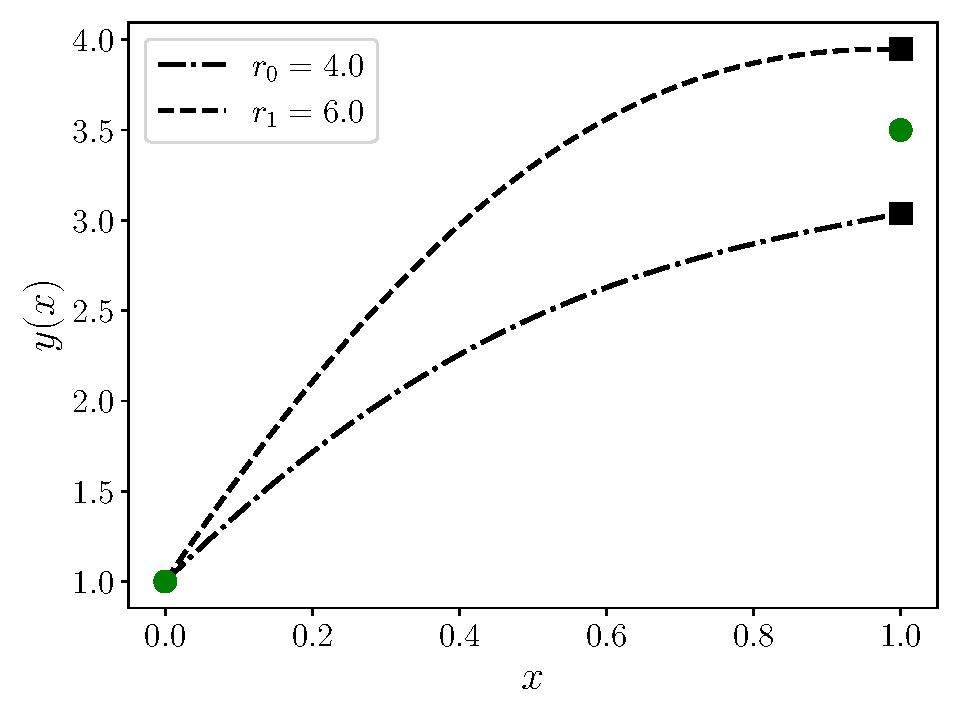
\includegraphics[height=0.5\textheight]{code/disparo-pre.pdf}
\end{center}
\end{frame}

\begin{frame}[fragile]
\begin{columns}
\cw{0.45}
\pycode[firstline=15, lastline=20]{code/disparo.py}
\pycode[firstline=36, lastline=42]{code/disparo.py}

\begin{shell}
$ ./disparo.py 
      converged: True
           flag: 'converged'
 function_calls: 42
     iterations: 40
           root: 5.016654027140248
\end{shell}
\pause

\cw{0.45}
\begin{center}
   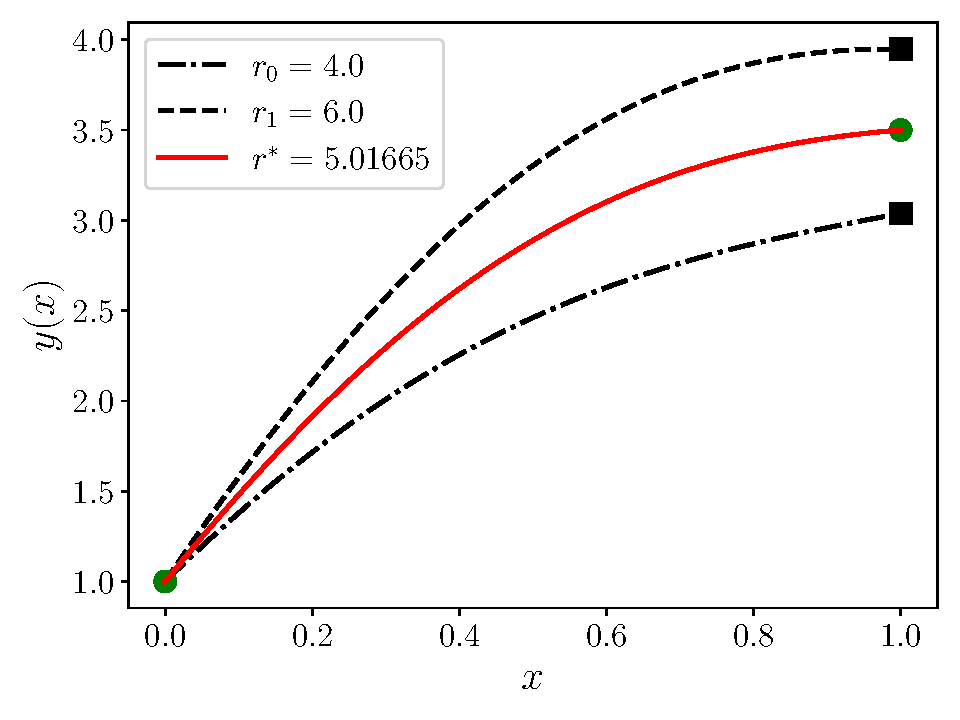
\includegraphics[width=0.9\textwidth]{code/disparo.pdf}
\end{center}
\end{columns}
\end{frame}

\begin{frame}  % Brian Bradie Sec. 8.1 pg. 674
%\begin{columns}[t]
%\cx
\textbf{Diferencias finitas:} aproximación de derivadas por diferencias finitas. Problema lineal con valores de contorno:
\begin{equation} y'' = p(x) y' + q(x) y + r(x), \; a \leq x \leq b, \; y(a) = \alpha, \, y(b) = \beta \label{eq:plineal} \end{equation} \pause
\vspace{-1.0em}

\textbf{Malla:} dividimos $[a, b]$ en $N$ subintervalos:
\begin{center}
    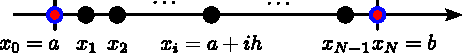
\includegraphics[scale=1.0]{figs/grilla-1d.pdf}
\end{center}
con $h = (b-a)/N$, $x_i = a + ih, i = 0, 1, \ldots, N-1, N$. \pause

Expansión de $y$: polinomio de Taylor, alrededor de $x_i$ evaluando en $x_{i+1}$ y $x_{i-1}$, con $y \in C^4[x_{i-1}, x_{i+1}]$:
\begin{align*}
    y(x_i+h) &= y(x_i) + h y'(x_i) + \frac{h^2}{2} y''(x_i) + \frac{h^3}{6} y'''(x_i) + \frac{h^4}{24} y^{(4)}(\xi_i^+) \\
    y(x_i-h) &= y(x_i) - h y'(x_i) + \frac{h^2}{2} y''(x_i) - \frac{h^3}{6} y'''(x_i) + \frac{h^4}{24} y^{(4)}(\xi_i^-) 
\end{align*}
con $\xi_i^+ (x_i, x_i+h)$ y $\xi_i^- \in (x_i - h, x_i)$. Restando y sumando: \vspace{-0.5em}
\begin{columns}
\cw{0.6}
\begin{equation}
    \begin{split}
    y'(x_i) &=\frac{1}{2h} [y(x_{i+1}) - y(x_{i-1})] - \frac{h^2}{6} y'''(\eta_i) \\
y''(x_i) &= \frac{1}{h^2} [ y(x_{i+1}) - 2 y(x_i) + y(x_{i-1})] - \frac{h^2}{12} y^{(4)}(\xi_i)
\end{split}
\label{eq:diffin}
\end{equation}
\cw{0.3}
con $\eta_i, \xi_i \in (x_{i-1}, x_{i+1})$. 
Notación: $y(x_i) \mapsto y_i$, $f(x_i) \mapsto f_i, f = p, q, r$.
\end{columns}
\end{frame}

\begin{frame}
Reemplazando \eqref{eq:diffin} en \eqref{eq:plineal}:
\[
\frac{y_{i+1} - 2 y_i + y_{i-1}}{h^2} = p_{i} \left[\frac{y_{i+1} - y_{i-1}}{2h}\right] + q_i y_i + r_i - \frac{h^2}{12}[2 p_i y'''(\eta_i) - y^{(4)}(\xi_i)] \]
\pause

Condiciones de borde $y_0 = \alpha, \, y_{N + 1} = \beta$, error de truncamiento $\bigO(h^2)$ $\mapsto$ sistema de ecuaciones lineales:
\[ \left(\frac{-y_{i+1} + 2 y_i - y_{i-1}}{h^2}\right) + p(x_i) \left(\frac{y_{i+1} - y_{i-1}}{2 h}\right) + q(x_i) y_i = -r(x_i) \]
para los puntos interiores de la malla $i = 1, 2, \ldots, N - 1$. Reordenando:
\[ -\left(1 + \frac{h}{2}p_i\right) y_{i-1} + \left(2 + h^2 q_i \right) y_i - \left(1 - \frac{h}{2} p_i \right) y_{i+1} = -h^2 r(x_i) \]
\begin{columns}[t]
\cx
Sistema con matriz tridiagonal $(N - 1) \mul (N - 1)$:
\[ \bm{A} \bm{y} = \bm{b} \]

\cx
Para $i = 1$: 
\[ y_{i-1} = y_0 = y(a) = \alpha \]
Para $i = N-1$:
\[ y_{i + 1} = y_N = y(b) = \beta \]
\end{columns}
\end{frame}

\begin{frame}
    \[ \bm{A} = \begin{bmatrix}
        2 + h^2 q_1 & -1 + \frac{h}{2} p_1 & & & & & \text{\Huge 0} \\
        -1-\frac{h}{2} p_2 & 2 + h^2 q_2 & -1 +\frac{h}{2} p_2 & & & \\
                              & -1-\frac{h}{2} p_3 & 2 + h^2 q_3 & -1 +\frac{h}{2} p_3  & & \\
                              & & & \ddots &  & & \\
                              & & && -1-\frac{h}{2} p_{N-2} & 2 + h^2 q_{N-2} & -1 +\frac{h}{2} p_{N-2} \\
        \text{\Huge 0}              & & & & & -1 - \frac{h}{2} p_{N-1} & 2 + h^2 q_{N-1}
    \end{bmatrix} \]
    \[ \bm{y} = \begin{bmatrix} y_1 \\ y_2 \\ \vdots \\ y_{N-2} \\ y_{N-1} \end{bmatrix}, \quad 
    \bm{b} = \begin{bmatrix} 
        -h^2 r_1 + \left(1 + \frac{h}{2} p_1 \right) \alpha \\
        -h^2 r_2 \\
        \vdots \\
    -h^2 r_{N-2} \\
    -h^2 r_{N-1} + \left(1 - \frac{h}{2} p_{N-1} \right) \beta
\end{bmatrix} 
    \]
\end{frame}

\begin{frame}
\begin{columns}[t]
\cw{0.4}
\textbf{Ejemplo:}
\[ \begin{split} y'' = 12 x - 4 y, \; 0 \leq x \leq 1 \\ y(0) = 1,\; y(1) = 3.5 \end{split} \]
\pycode[firstline=7, lastline=21]{code/diferencias-finitas.py}

\cw{0.5}
\pycode[firstline=22, lastline=44]{code/diferencias-finitas.py}
\end{columns}
\end{frame}

\begin{frame}[fragile]
    \begin{columns}
\cw{0.3}
\pycode[firstline=46]{code/diferencias-finitas.py}

\cw{0.6}
\begin{shell}
N = 10
x =  [0.  0.1 0.2 0.3 0.4 0.5 0.6 0.7 0.8 0.9 1. ] h =  0.1
[[ 1.96 -1.    0.    0.    0.    0.    0.    0.    0.  ]
 [-1.    1.96 -1.    0.    0.    0.    0.    0.    0.  ]
 [ 0.   -1.    1.96 -1.    0.    0.    0.    0.    0.  ]
 [ 0.    0.   -1.    1.96 -1.    0.    0.    0.    0.  ]
 [ 0.    0.    0.   -1.    1.96 -1.    0.    0.    0.  ]
 [ 0.    0.    0.    0.   -1.    1.96 -1.    0.    0.  ]
 [ 0.    0.    0.    0.    0.   -1.    1.96 -1.    0.  ]
 [ 0.    0.    0.    0.    0.    0.   -1.    1.96 -1.  ]
 [ 0.    0.    0.    0.    0.    0.    0.   -1.    1.96]]
b =  [ 1.    -0.012 -0.024 -0.036 -0.048 -0.06  -0.072 -0.084  3.392]
\end{shell}
\end{columns}
\end{frame}

\begin{frame}
\begin{center}
    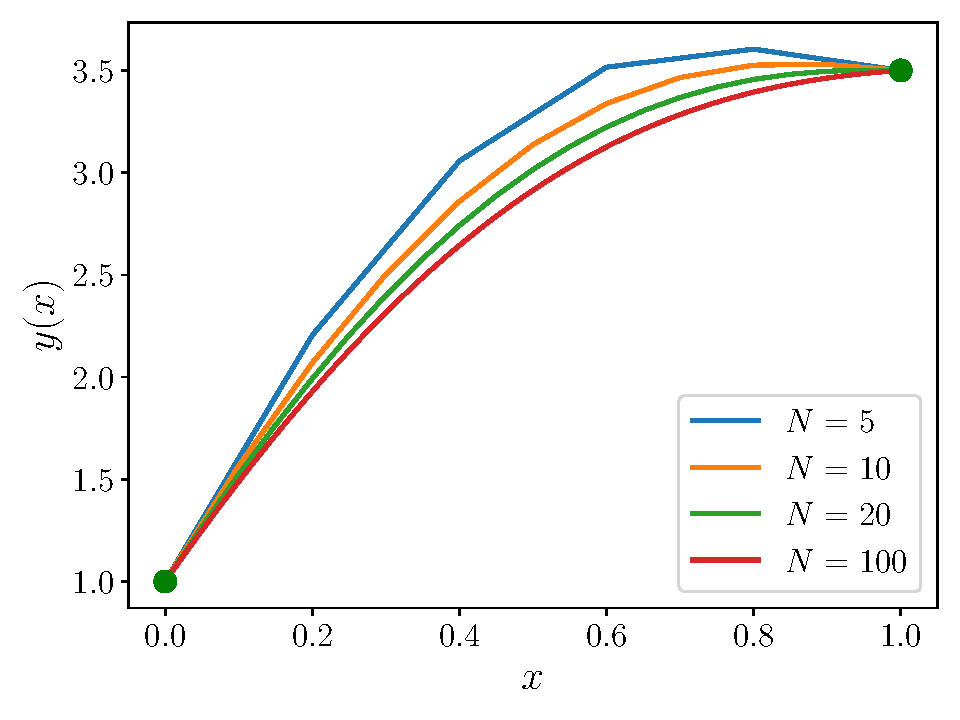
\includegraphics[scale=0.6]{code/dif-finitas.pdf}
\end{center}
\end{frame}

\section*{Bibliografía}
\begin{frame}[allowframebreaks]{Lecturas recomendadas}
\begin{itemize}
    \item \fullcite{burden2017}. Capítulo 11.
    \item \fullcite{bradie2006}. Capítulo 8.
    \item \fullcite{kiusalaas2013}. Capítulo 8.
    \item \fullcite{mathews2004}. Capítulo 9.
\end{itemize}
\end{frame}

\end{document}

